\documentclass[laboratorio]{guia}

\def \practnum {5} 
\def \practica {Circuito RC: reg\'\i menes transitorio y estacionario}

\def \materia {Laboratorio de F\'\i sica II para Qu\'\i micos}
\def \periodo {2do. Cuatrimestre de 2015}
\def \catedra {Pablo Cobelli}
\def \website {http://materias.df.uba.ar/f2qa2015c2}
 
\usepackage{graphics}
\usepackage{amsmath}
\usepackage{amsfonts}
\usepackage{graphicx}
\usepackage{float}
\usepackage{wrapfig}
\usepackage{subfigure}
\usepackage{bm}
\usepackage{grffile}
\usepackage{color}
\usepackage{framed}
\usepackage[utf8]{inputenc}
\usepackage[T1]{fontenc}
\usepackage{lmodern}
\usepackage{circuitikz}
\usepackage[spanish]{babel}
\usepackage{babelbib}
\selectbiblanguage{spanish}

 

%----------------------------------------------------------
% Agrega al path de figuras el subdirectorio con el mismo
%     nombre que el archivo principal del proyecto
\graphicspath{{./\jobname/}}

%----------------------------------------------------------
% Definicion del entorno 'sabermas'
\makeatletter
\definecolor{shadecolor}{rgb}{0.89,0.91,0.94}
\newenvironment{sabermas}[1]{%
\vfill
\begin{shaded}
  \begin{center}
  {\textsection{Para saber m\'as}}
  \end{center}
  #1
\sf } 
{%
\end{shaded}%
}
\makeatother

%----------------------------------------------------------
% Definicion del entorno 'problema'
\newcounter{ContadorProblema}
\setcounter{ContadorProblema}{0}
\newcounter{TieneFiguraAsociada}
\setcounter{TieneFiguraAsociada}{0}
\newcounter{UbicacionFigura}
\setcounter{UbicacionFigura}{0}

\newenvironment{problema}[2][]
{%
    \ifx\relax#1\relax%
        \setcounter{TieneFiguraAsociada}{0}
        \else
        \setcounter{TieneFiguraAsociada}{1}
    \fi
    \def \archivofigura {#1}
    % 
    \refstepcounter{ContadorProblema}
    \noindent%
    \ifnum\value{TieneFiguraAsociada} < 1%
        {\sffamily \bfseries Problema \arabic{ContadorProblema}.}
        %{\sc {#1}}%
        \par\nobreak\par\nobreak%
        \medskip 
    \else
        % Va con figura; resta determinar de que lado.
        \ifnum\value{UbicacionFigura} < 1
            % Poner la figura del lado derecho
            \begin{minipage}{12.25cm}
            {\sffamily \bfseries Problema \arabic{ContadorProblema}.}
            %{\sc {#1}}%
            \par\nobreak\par\nobreak%
            \medskip 
        \else
            % Poner la figura del lado izquierdo
            \begin{minipage}{4.5cm}
                \centering
                \includegraphics[width=4.5cm]{\archivofigura}
                {\footnotesize {\sffamily Esquema asociado al 
                problema \arabic{ContadorProblema}}.}
            \end{minipage}\hfill%
            \begin{minipage}{12.25cm}
                {\sffamily \bfseries Problema \arabic{ContadorProblema}.}
                %{\sc {#1}}%
                \par\nobreak\par\nobreak%
                \medskip 
        \fi
    \fi
}
{%
    \ifnum\value{TieneFiguraAsociada} < 1%
        % \par \bigskip \vskip 0.3cm
    \else
        % Va con figura; resta determinar de que lado.
        \ifnum\value{UbicacionFigura} < 1
            % Poner la figura del lado derecho
            \end{minipage}\hfill%
            \begin{minipage}{4.5cm}
                \centering
                \includegraphics[width=4.5cm]{\archivofigura}
                {\footnotesize {\sffamily Esquema asociado al 
                problema \arabic{ContadorProblema}}.}
            \end{minipage}
        \else
            % Poner la figura del lado izquierdo
            \end{minipage}%
        \fi
    \fi
    \setcounter{TieneFiguraAsociada}{0}
    \par \bigskip \vskip 0.3cm
    % Permutamos el valor de la ubicacion
    \ifnum\value{UbicacionFigura} < 1
        \setcounter{UbicacionFigura}{1}
    \else
        \setcounter{UbicacionFigura}{0}
    \fi
}

%----------------------------------------------------------
% Definicion/Redefinicion de estilos
\renewcommand{\vec}[1]{\ensuremath{\mathbf{#1}}}



\hyphenation{ coe-fi-cien-tes coe-fi-cien-te au-to-va-lor
              au-to-va-lo-res co-rres-pon-der pro-ble-ma 
              cual-quie-ra po-la-ri-za-cio-nes }

\graphicspath{{./Guia_05_Circuito_RC/}}

\begin{document} 
\objetivo{Estudiar los comportamientos de un circuito RC en dos reg\'\i menes de operaci\'on 
    distintos: (a) transitorio y (b) estacionario. Para el transitorio, se
    propone estudiar los procesos de carga y descarga de un capacitor en un
    circuito RC. Caracterizar ambos determinando qu\'e tipo de evoluc\'on
    temporal presentan, y midiendo los tiempos caracter\'\i sticos asociados
    a cada uno de ellos. Para el estacionario, se busca determinar la respuesta
    del circuito al excitarlo con una se\~nal peri\'odica, variando la
    frecuencia de trabajo del sistema.
    \tematicas{Circuitos de corrientes variables en el tiempo, RC, carga y
        descarga de un capacitor, tiempo caracter\'\i stico, filtros pasaaltos y
    pasabajos}} 
\maketitle

\section{Introducci\'on}

Considere el circuito RC mostrado en la Figura \ref{fig:circuitoRC}, en el
cual el capacitor se encuentra completamente descargado inicialmente y la
llave S, abierta. Al cerrarse esta \'ultima, la diferencia de potencial
$V$ impuesta por la fuente genera una corriente $I$ en el circuito. Esta 
corriente tendr\'a el efecto de llevar cargas de signo opuesto a las caras 
del capacitor. Resulta intuitivo que esta corriente no ser\'a constante en el tiempo; 
en particular esperamos que la misma se anule cuando el capacitor se haya
cargado. 


Un capacitor de capacidad $C$ conectado a una fuente de tensi\'on $V$ constante 
adquiere una carga $q = C V$. Esto nos permite conocer la ca\'\i da de
potencial sobre nuestro capacitor. Por otro lado, la ecuaci\'on circuital para
el circuito RC resulta simplemente:

\begin{equation}
    V = RI + \frac{q}{C},
\end{equation}
donde tanto la corriente $I$ como la carga $q$ est\'an variando instante a
instante, es decir que $I \equiv I(t)$ y $q \equiv q(t)$. Recordemos, por otro
lado, que tanto la tensi\'on $V$ de la fuente, la resistencia $R$ del resistor
y la capacidad $C$ del capacitor son constantes, dado que describen propiedades de
cada uno de dichos elementos. Empleando ahora la definici\'on de corriente,

$$ I = \frac{dq}{dt}, $$
podemos reescribir la \'ultima ecuaci\'on en t\'erminos de una \'unica
funci\'on inc\'ognita, ya sea $q(t)$ o $I(t)$. Vamos a elegir reexpresarla en
funci\'on de $q(t)$, de lo que se obtiene

\begin{equation}
    V = R \frac{dq}{dt}(t) + \frac{1}{C} q(t).
    \label{eq:ecuacionRC}
\end{equation}

Esta ecuaci\'on es una ecuaci\'on diferencial ordinaria de orden 1 para $q(t)$, 
cuya soluci\'on nos dar\'a la evoluci\'on temporal (desde un instante inicial
dado) de la carga en el capacitor. 
Para resolverla, debemos especificar adem\'as una condici\'on inicial para la 
carga $q(t)$ en el capacitor. Dado que estamos considerando el caso en el que
el mismo se encuentra inicialmente descargado, tenemos
\begin{equation}
    q(t=0) = 0,
\end{equation}
como condici\'on inicial para el proceso de carga. 

La ecuaci\'on diferencial en derivadas totales para $q(t)$ dada por
\eqref{eq:ecuacionRC} tiene una soluci\'on general de la forma:
\begin{equation}
    q(t) = A \text{e}^{-t/\tau} + CV,
\end{equation}
donde $\tau = RC$ es el tiempo caracter\'\i stico del circuito RC, y la
constante $A$ se determina de las condiciones del problema particular que se
est\'e considerando. Por ejemplo, si el capacitor esta inicialmente descargado,
resulta f\'acil obtener que $A = -CV$, por lo que
\begin{equation*}
    q(t) = CV \left(1 - \text{e}^{-t/\tau} \right),
\end{equation*}
por lo que la corriente en funci\'on del tiempo resulta
\begin{equation*}
    I(t) = \frac{V}{R} \text{e}^{-t/\tau}.
\end{equation*}

En base a esto, plantee c\'omo ser\'\i an las ecuaciones que describen la
descarga del capacitor, reemplazando para ello la fuente por un cortocircuito.


% \begin{figure}[t!]
    % \centering
    % \begin{tikzpicture}
        -- Circuito RC -- % \draw[step=0.5, very thin, black!20] (-1, -0.5) grid (6, 2.5);
        % \path (0, 0) coordinate (ref_gnd);
        % \draw
          % (ref_gnd) to[battery1=\(V\)] ++(0,2)
                    % to[R=\(R\)] ++(3,0) 
                    % to[C=\(C\)] ++(0,-2) 
          % -- (ref_gnd);
    % \end{tikzpicture}
    % \vspace{0.5cm}
    % \caption{Esquema del circuito RC empleado.}
    % \label{fig:circuitoRC}
% \end{figure}

\begin{figure}[t!]
    \centering
    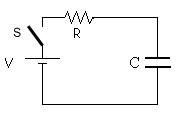
\includegraphics[width=6cm]{LG05--000.png}
    \caption{Esquema del circuito RC empleado.}
    \label{fig:circuitoRC}
\end{figure}

\section{Carga y descarga de un capacitor}

En esta primera etapa se estudia el proceso de carga y descarga del capacitor. 

\subsection{Midiendo en forma manual con mult\'\i metro}

De realizar la experiencia con cron\'ometro, se sugiere elegir valores de $R$ y
$C$ de manera tal que el producto $RC$ sea igual o superior a 100 segundos. De
esta forma los procesos de carga y descarga son lo sufientemente lentos como
para poder tomar los datos manualmente. 

\subsection{Midiendo a trav\'es de la placa de adquisici\'on SensorDAQ}

En cualquiera de las dos modalidades que se elija medir, se busca responder
las siguientes preguntas:
\begin{itemize}
    \item Cu\'al es el tiempo caracter\'\i stico (de carga y descarga) que se 
        obtiene de las  mediciones? Es el mismo para ambos procesos?
    \item Cu\'al es el valor de tensi\'on que se alcanza al llegar al 
        r\'egimen estacionario? 
    \item En el proceso de descarga, sobre que elemento disipativo se 
        descarga el capacitor?
    \item Es posible estimar la resistencia interna del mult\'\i metro? 
\end{itemize}

Repetir las mediciones utilizando otro valor de tensi\'on de trabajo $V'$
para la fuente. Observa cambios en el tiempo caracter\'\i stico producto de
esta modificaci\'on?

\section{Respuesta estacionaria}

En esta parte de la pr\'actica reemplazaremos la fuente de tensi\'on 
constante por una de tensi\'on alterna. Estudiaremos la respuesta del sistema
cuando se excita con distintas frecuencias. Para ello se utiliza un generador
de funciones como fuente de tensi\'on alterna y un osciloscopio para medir
las se\~nales de inter\'es. 

\subsection{Filtro pasabajos; circuito integrador}

Para esta instancia se sugieren elegir valores de $R$ y $C$ de manera que 
su producto sea del orden de 100~$\mu$s. Aplicando una se\~nal sinusoidal de
amplitud de 5 Volts, estudie la respuesta del sistema en funci\'on de la
frecuencia. 

Grafique luego el cociente entre las amplitudes de la se\~nal de salida y
la de entrada como funci\'on de la frecuencia $f = \omega/(2\pi)$. Intente 
determinar el desfasaje $\phi$ entre la se\~nal de entrada y la de salida; que 
puede definirse como $\phi = \omega \Delta t$. Estudie como var\'\i a este 
desfasaje en funci\'on de la frecuencia $f$. 

A continuaci\'on cambie la forma de onda de la se\~nal de entrada a una 
onda cuadrada. Nuevamente, estudie la forma de la se\~nal de salida en 
funci\'on de la frecuencia. Existe alguna relaci\'on entre ambas? Intente
describir mediante los modelos propuestos los resultados experimentales 
obtenidos. 

\subsection{Filtro pasaaltos; circuito derivador}

Repita las mediciones tomadas en el caso anterior, pero esta vez midiendo 
la diferencia de tensi\'on (o ca\'\i da de potencial) sobre el resistor. 
Discuta las similitudes y diferencias. 

\nocite{Alonso1998,Purcell1988,Reitz1996,Trelles1984,Reitz1996}
\bibliographystyle{unsrt} 
\bibliography{Bibliografia}

\end{document}
